\documentclass{rapportENSET}

% Encoding + language
\usepackage[utf8]{inputenc}
\usepackage[T1]{fontenc}
% babel is already loaded by rapportENSET.cls

% Core packages
\usepackage{graphicx}
\usepackage{float}
\usepackage{xcolor}
\usepackage{geometry}
\usepackage{amsmath, amssymb}
\usepackage{enumitem}
\usepackage{fancyhdr}
\usepackage{tikz}
\usetikzlibrary{shapes.geometric, arrows, positioning, fit, backgrounds}
\usepackage{tcolorbox}
\usepackage{caption}
\usepackage{pifont}
\usepackage{listings}
\usepackage{tabularx}
\usepackage{booktabs}
\usepackage{longtable}
\usepackage{multirow}
\usepackage{hyperref}

% -----------------------------------------------------------
% Colors
% -----------------------------------------------------------

\definecolor{winblue}{RGB}{0,120,215}
\definecolor{awsorange}{RGB}{255,153,0}
\definecolor{wazuhblue}{RGB}{0,125,166}
\definecolor{alertred}{RGB}{220,53,69}
\definecolor{successgreen}{RGB}{40,167,69}
\definecolor{codebg}{RGB}{245,245,245}
\definecolor{codeframe}{RGB}{200,200,200}

% -----------------------------------------------------------
% Custom item bullets
% -----------------------------------------------------------

\newcommand{\bulletpoint}{\textcolor{winblue}{\textbullet}}
\renewcommand{\labelitemi}{\bulletpoint}

% -----------------------------------------------------------
% Code listing style
% -----------------------------------------------------------

\lstdefinestyle{wazuhquery}{
    backgroundcolor=\color{codebg},
    basicstyle=\ttfamily\small,
    breaklines=true,
    frame=single,
    framesep=5pt,
    rulecolor=\color{codeframe},
    xleftmargin=10pt,
    xrightmargin=10pt,
}

% -----------------------------------------------------------
% Alert box
% -----------------------------------------------------------

\newtcolorbox{alertbox}[1][]{
    colback=red!5!white,
    colframe=alertred,
    fonttitle=\bfseries,
    title=#1
}

\newtcolorbox{infobox}[1][]{
    colback=blue!5!white,
    colframe=wazuhblue,
    fonttitle=\bfseries,
    title=#1
}

% -----------------------------------------------------------

\title{Wazuh SIEM/EDR Cloud Lab}

\begin{document}

%----------- Informations du rapport ---------

\titre{Wazuh SIEM/EDR Cloud Lab Implementation}
\sujet{Module : Cloud Computing}
\enseignant{Prof. Azeddine \textsc{KHIAT}}
\eleves{Yasser \textsc{NAMEZ}}

%----------- Initialisation -------------------

\fairemarges
\fairepagedegarde
\tabledematieres
\newpage

%------------ Corps du rapport ----------------

% ============================================================
% SECTION 1: ARCHITECTURE
% ============================================================

\section{Architecture VPC + Security Groups + EC2 Instances}

\subsection{Overview}

This section describes the cloud infrastructure deployed on AWS for the Wazuh SIEM/EDR lab environment. The architecture follows security best practices with network segmentation and least-privilege access controls.

\subsection{AWS VPC Configuration}

\begin{figure}[H]
\centering
\includegraphics[width=0.95\textwidth]{../screenshots/VCP.png}
\caption{AWS VPC Configuration - 10.0.0.0/16}
\label{fig:vpc}
\end{figure}

\begin{figure}[H]
\centering
\includegraphics[width=0.95\textwidth]{../screenshots/subnets.png}
\caption{VPC Subnets Configuration}
\label{fig:subnets}
\end{figure}

\subsection{EC2 Instances}

\begin{figure}[H]
\centering
\includegraphics[width=0.95\textwidth]{../screenshots/Instances running init.png}
\caption{All EC2 Instances Running}
\label{fig:instances-running}
\end{figure}

\subsubsection{Wazuh Server Instance}

\begin{figure}[H]
\centering
\includegraphics[width=0.95\textwidth]{../screenshots/Instance summary for i-02b3d23c6fdce738d (Wazuh-Server).png}
\caption{Wazuh-Server Instance Details (Ubuntu 22.04, t3.large)}
\label{fig:wazuh-server}
\end{figure}

\subsubsection{Linux Client Instance}

\begin{figure}[H]
\centering
\includegraphics[width=0.95\textwidth]{../screenshots/Instance summary for i-07c2a03addeeac5d2 (Linux-Client).png}
\caption{Linux-Client Instance Details (Ubuntu 22.04, t2.micro)}
\label{fig:linux-client}
\end{figure}

\subsubsection{Windows Client Instance}

\begin{figure}[H]
\centering
\includegraphics[width=0.95\textwidth]{../screenshots/Instance summary for i-083a06098143e6e5e (Windows-Client).png}
\caption{Windows-Client Instance Details (Windows Server 2022, t2.medium)}
\label{fig:windows-client}
\end{figure}

\subsection{Security Groups Configuration}

\subsubsection{Wazuh Server Security Group}

\begin{figure}[H]
\centering
\includegraphics[width=0.95\textwidth]{../screenshots/sg-013b8487893e74ae4 - Wazuh-Server-SG.png}
\caption{Wazuh-Server-SG: Inbound Rules (Ports 22, 443, 1514, 1515)}
\label{fig:wazuh-sg}
\end{figure}

\subsubsection{Wazuh Clients Security Group}

\begin{figure}[H]
\centering
\includegraphics[width=0.95\textwidth]{../screenshots/sg-0be305e637154660d - Wazuh-Clients-SG.png}
\caption{Wazuh-Clients-SG: Inbound Rules (SSH 22, RDP 3389)}
\label{fig:clients-sg}
\end{figure}

\subsection{Network Architecture Diagram}

\begin{figure}[H]
\centering
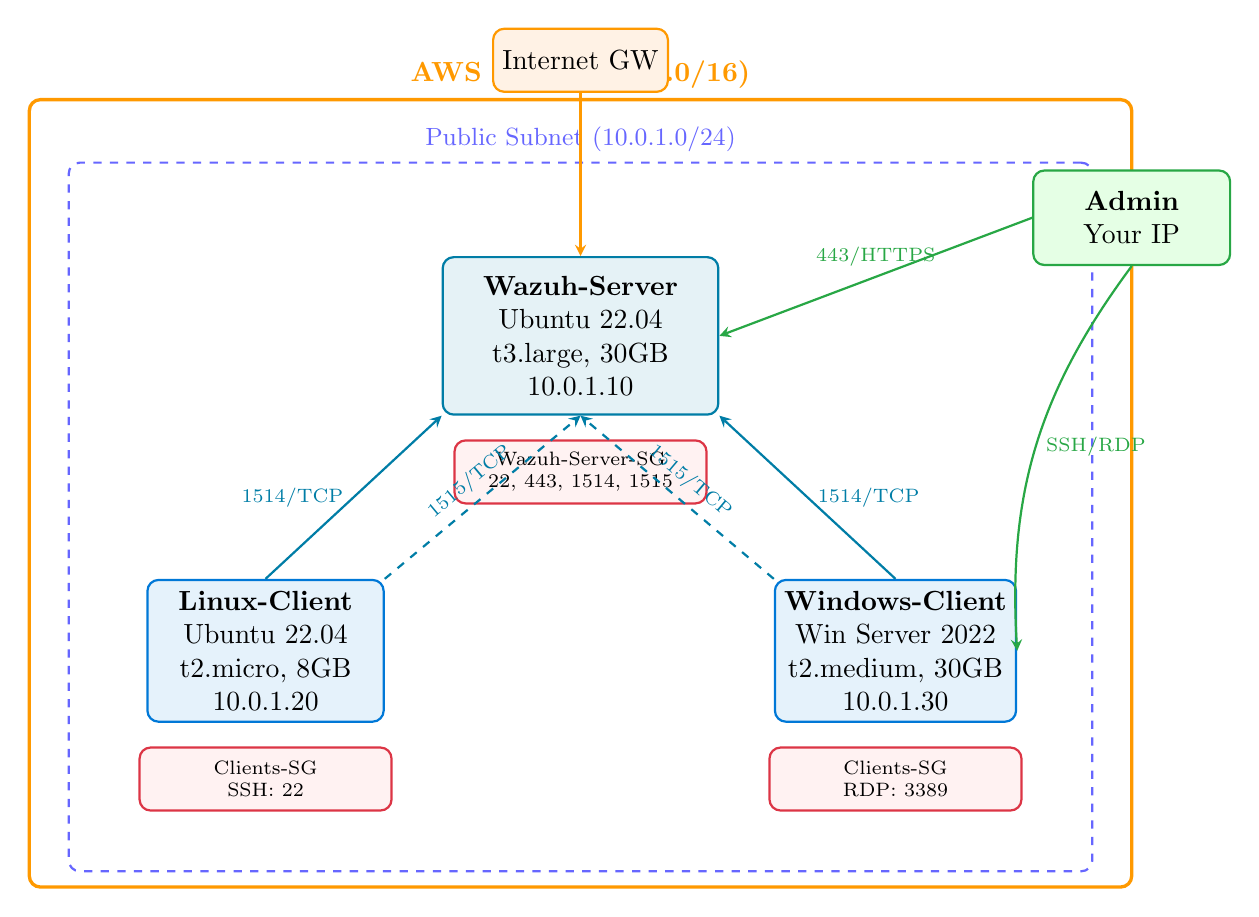
\begin{tikzpicture}[
    node distance=1.5cm,
    vpc/.style={draw=awsorange, very thick, rounded corners, minimum width=14cm, minimum height=10cm},
    subnet/.style={draw=blue!60, dashed, thick, rounded corners, minimum width=13cm, minimum height=9cm},
    server/.style={draw=wazuhblue, fill=wazuhblue!10, thick, rounded corners, minimum width=3.5cm, minimum height=2cm, align=center},
    client/.style={draw=winblue, fill=winblue!10, thick, rounded corners, minimum width=3cm, minimum height=1.8cm, align=center},
    sg/.style={draw=alertred, fill=red!5, thick, rounded corners, minimum width=3.2cm, minimum height=0.8cm, align=center, font=\scriptsize},
    arrow/.style={->, thick, >=stealth},
    admin/.style={draw=successgreen, fill=green!10, thick, rounded corners, minimum width=2.5cm, minimum height=1.2cm, align=center}
]

% VPC
\node[vpc, label={[awsorange, font=\bfseries]above:AWS VPC (10.0.0.0/16)}] (vpc) {};

% Subnet
\node[subnet, label={[blue!60, font=\small]above:Public Subnet (10.0.1.0/24)}] at (0,-0.3) (subnet) {};

% Wazuh Server
\node[server] at (0,2) (wazuh) {\textbf{Wazuh-Server}\\Ubuntu 22.04\\t3.large, 30GB\\10.0.1.10};

% Security Group for Wazuh
\node[sg, below=0.3cm of wazuh] (wazuhsg) {Wazuh-Server-SG\\22, 443, 1514, 1515};

% Linux Client
\node[client] at (-4,-2) (linux) {\textbf{Linux-Client}\\Ubuntu 22.04\\t2.micro, 8GB\\10.0.1.20};

% Windows Client
\node[client] at (4,-2) (windows) {\textbf{Windows-Client}\\Win Server 2022\\t2.medium, 30GB\\10.0.1.30};

% Security Groups for Clients
\node[sg, below=0.3cm of linux] (linuxsg) {Clients-SG\\SSH: 22};
\node[sg, below=0.3cm of windows] (winsg) {Clients-SG\\RDP: 3389};

% Admin
\node[admin] at (7,3.5) (admin) {\textbf{Admin}\\Your IP};

% Internet Gateway
\node[draw=awsorange, fill=orange!10, thick, rounded corners, minimum width=2cm, minimum height=0.8cm] at (0,5.5) (igw) {Internet GW};

% Arrows - Agent Communication
\draw[arrow, wazuhblue] (linux.north) -- node[left, font=\scriptsize] {1514/TCP} (wazuh.south west);
\draw[arrow, wazuhblue] (windows.north) -- node[right, font=\scriptsize] {1514/TCP} (wazuh.south east);

% Arrows - Enrollment
\draw[arrow, dashed, wazuhblue] (linux.north east) -- node[above, font=\scriptsize, sloped] {1515/TCP} (wazuh.south);
\draw[arrow, dashed, wazuhblue] (windows.north west) -- node[above, font=\scriptsize, sloped] {1515/TCP} (wazuh.south);

% Admin connections
\draw[arrow, successgreen] (admin.west) -- node[above, font=\scriptsize] {443/HTTPS} (wazuh.east);
\draw[arrow, successgreen, bend right=20] (admin.south) to node[right, font=\scriptsize] {SSH/RDP} (windows.east);

% Internet
\draw[arrow, awsorange] (igw.south) -- (wazuh.north);

\end{tikzpicture}
\caption{Wazuh SIEM/EDR Lab Architecture Diagram}
\label{fig:architecture}
\end{figure}

\subsection{Connectivity Testing}

\subsubsection{SSH to Wazuh Server}

\begin{figure}[H]
\centering
\includegraphics[width=0.95\textwidth]{../screenshots/Test SSH to Wazuh-Server.png}
\caption{SSH Connection Test to Wazuh-Server}
\label{fig:ssh-wazuh}
\end{figure}

\subsubsection{SSH to Linux Client}

\begin{figure}[H]
\centering
\includegraphics[width=0.95\textwidth]{../screenshots/Test SSH to Linux-Client.png}
\caption{SSH Connection Test to Linux-Client}
\label{fig:ssh-linux}
\end{figure}

\subsubsection{RDP to Windows Client}

\begin{figure}[H]
\centering
\includegraphics[width=0.95\textwidth]{../screenshots/Test RDP to Windows-Client.png}
\caption{RDP Connection Test to Windows-Client}
\label{fig:rdp-windows}
\end{figure}

\subsection{Infrastructure Summary}

\begin{table}[H]
\centering
\begin{tabularx}{\textwidth}{|l|X|l|l|l|}
\hline
\textbf{Instance} & \textbf{Operating System} & \textbf{Type} & \textbf{Storage} & \textbf{Private IP} \\
\hline
Wazuh-Server & Ubuntu 22.04 LTS & t3.large & 30 GB & 10.0.1.10 \\
\hline
Linux-Client & Ubuntu 22.04 LTS & t2.micro & 8 GB & 10.0.1.20 \\
\hline
Windows-Client & Windows Server 2022/2025 & t2.medium & 30 GB & 10.0.1.30 \\
\hline
\end{tabularx}
\caption{EC2 Instance Specifications}
\label{tab:instances}
\end{table}

\begin{infobox}[Security Best Practices Implemented]
\begin{itemize}
    \item All agent-to-server communication uses private IP addresses within the VPC
    \item Management ports are restricted to specific administrator IP addresses
    \item Security groups follow the principle of least privilege
    \item Encrypted communication channels for all sensitive traffic
    \item Network segmentation isolates the monitoring infrastructure
\end{itemize}
\end{infobox}

\newpage

% ============================================================
% SECTION 2: WAZUH SETUP AND DASHBOARD
% ============================================================

\section{Wazuh Server Setup and Dashboard}

\subsection{Wazuh Services Status}

\begin{figure}[H]
\centering
\includegraphics[width=0.95\textwidth]{../screenshots/Wazuh services.png}
\caption{Wazuh Services Running on Server}
\label{fig:wazuh-services}
\end{figure}

\begin{figure}[H]
\centering
\includegraphics[width=0.95\textwidth]{../screenshots/wazuh-services-running.png}
\caption{Wazuh Services Status Verification}
\label{fig:wazuh-services-running}
\end{figure}

\subsection{Wazuh Dashboard Access}

\begin{figure}[H]
\centering
\includegraphics[width=0.95\textwidth]{../screenshots/wazuh-dashboard.png}
\caption{Wazuh Dashboard Login Interface}
\label{fig:wazuh-dashboard-login}
\end{figure}

\begin{figure}[H]
\centering
\includegraphics[width=0.95\textwidth]{../screenshots/dashboard 12.png}
\caption{Wazuh Dashboard Main Overview}
\label{fig:dashboard-overview}
\end{figure}

\begin{figure}[H]
\centering
\includegraphics[width=0.95\textwidth]{../screenshots/event dashboard.png}
\caption{Wazuh Security Events Dashboard}
\label{fig:event-dashboard}
\end{figure}

\subsection{Agent Enrollment and Status}

\subsubsection{Linux Agent Connection}

\begin{figure}[H]
\centering
\includegraphics[width=0.95\textwidth]{../screenshots/Agent is Running linux.png}
\caption{Linux Agent Running and Connected}
\label{fig:linux-agent-running}
\end{figure}

\subsubsection{Windows Agent Connection}

\begin{figure}[H]
\centering
\includegraphics[width=0.95\textwidth]{../screenshots/agent conneting windows.png}
\caption{Windows Agent Connecting to Wazuh Server}
\label{fig:windows-agent-connecting}
\end{figure}

\begin{figure}[H]
\centering
\includegraphics[width=0.95\textwidth]{../screenshots/Windows-Client-connecting.png}
\caption{Windows Client Agent Connection Status}
\label{fig:windows-client-connecting}
\end{figure}

\subsection{Active Agents Overview}

\begin{figure}[H]
\centering
\includegraphics[width=0.95\textwidth]{../screenshots/AGENT ACTIVE 1.png}
\caption{Active Agents Dashboard View 1}
\label{fig:agent-active-1}
\end{figure}

\begin{figure}[H]
\centering
\includegraphics[width=0.95\textwidth]{../screenshots/AGENT ACTIVE 2.png}
\caption{Active Agents Dashboard View 2 - Both Agents Connected}
\label{fig:agent-active-2}
\end{figure}

\begin{table}[H]
\centering
\begin{tabularx}{\textwidth}{|l|l|l|l|l|}
\hline
\textbf{Agent Name} & \textbf{IP Address} & \textbf{OS} & \textbf{Status} & \textbf{Version} \\
\hline
Linux-Client & 10.0.1.20 & Ubuntu 22.04 & \textcolor{successgreen}{\textbf{Active}} & 4.x \\
\hline
Windows-Client & 10.0.1.30 & Windows Server 2022 & \textcolor{successgreen}{\textbf{Active}} & 4.x \\
\hline
\end{tabularx}
\caption{Connected Agents Summary}
\label{tab:agents}
\end{table}

\newpage

% ============================================================
% SECTION 3: LINUX ALERTS
% ============================================================

\section{Security Events - Linux Client}

This section documents the security alerts captured from the Linux client (Ubuntu 22.04) demonstrating Wazuh's detection capabilities for common attack patterns and security events.

\subsection{Alert 1: SSH Brute Force Attack}

\begin{alertbox}[SSH Authentication Failure Detection]
\textbf{Rule IDs:} 5710, 5712, 5720 (Progressive Severity)\\
\textbf{Severity Level:} 5-10 (Medium to High)\\
\textbf{MITRE ATT\&CK:} T1110 - Brute Force
\end{alertbox}

\subsubsection{Attack Simulation}

\begin{figure}[H]
\centering
\includegraphics[width=0.95\textwidth]{../screenshots/SSH Brute Force Attack terminal.png}
\caption{SSH Brute Force Attack Simulation in Terminal}
\label{fig:ssh-brute-terminal}
\end{figure}

\subsubsection{Wazuh Detection}

\begin{figure}[H]
\centering
\includegraphics[width=0.95\textwidth]{../screenshots/SSH failed authentication.png}
\caption{SSH Failed Authentication Events Detected by Wazuh}
\label{fig:ssh-failed-auth}
\end{figure}

\subsubsection{Event Details}

\begin{table}[H]
\centering
\begin{tabularx}{\textwidth}{|l|X|}
\hline
\textbf{Attribute} & \textbf{Value} \\
\hline
Log Source & /var/log/auth.log \\
\hline
Event Type & SSH Authentication Failure \\
\hline
Detection Pattern & Multiple consecutive failed login attempts \\
\hline
Source IP & External attacker IP \\
\hline
Target User & root, admin, ubuntu (common usernames) \\
\hline
\end{tabularx}
\caption{SSH Brute Force Alert Details}
\end{table}

\subsubsection{Security Implication}

\begin{itemize}
    \item \textbf{Risk:} Potential unauthorized access attempt via credential guessing
    \item \textbf{Recommendation:} Implement fail2ban, use SSH key authentication, disable root login
    \item \textbf{Response:} Block source IP at firewall, review successful authentications
\end{itemize}

\subsection{Alert 2: Privilege Escalation (Sudo)}

\begin{alertbox}[Privilege Escalation Detection]
\textbf{Rule IDs:} 5402, 5401\\
\textbf{Severity Level:} 3-5 (Low to Medium)\\
\textbf{MITRE ATT\&CK:} T1548 - Abuse Elevation Control Mechanism
\end{alertbox}

\subsubsection{Wazuh Detection}

\begin{figure}[H]
\centering
\includegraphics[width=0.95\textwidth]{../screenshots/Successful sudo to ROOT executed.png}
\caption{Successful sudo to ROOT Execution Detected}
\label{fig:sudo-root}
\end{figure}

\begin{figure}[H]
\centering
\includegraphics[width=0.95\textwidth]{../screenshots/privileged rote.png}
\caption{Privileged Root Access Event Details}
\label{fig:privileged-root}
\end{figure}

\subsubsection{Event Details}

\begin{table}[H]
\centering
\begin{tabularx}{\textwidth}{|l|X|}
\hline
\textbf{Attribute} & \textbf{Value} \\
\hline
Log Source & /var/log/auth.log \\
\hline
Event Type & Successful sudo execution \\
\hline
User & ubuntu \\
\hline
Command & su (switch user to root) \\
\hline
Target User & ROOT \\
\hline
\end{tabularx}
\caption{Privilege Escalation Alert Details}
\end{table}

\subsubsection{Security Implication}

\begin{itemize}
    \item \textbf{Context:} May be legitimate administrative activity
    \item \textbf{Monitoring Value:} Critical for detecting unauthorized privilege escalation
    \item \textbf{Best Practice:} Implement just-in-time privilege access, log all sudo commands
\end{itemize}

\subsection{Alert 3: File Integrity Monitoring (FIM)}

\begin{alertbox}[File Integrity Change Detection]
\textbf{Rule IDs:} 550, 553\\
\textbf{Severity Level:} 7 (High)\\
\textbf{MITRE ATT\&CK:} T1078 - Valid Accounts, T1136 - Create Account
\end{alertbox}

\subsubsection{Event Details}

\begin{table}[H]
\centering
\begin{tabularx}{\textwidth}{|l|X|}
\hline
\textbf{Attribute} & \textbf{Value} \\
\hline
Detection Module & Syscheck (File Integrity Monitoring) \\
\hline
Monitored File & /etc/passwd \\
\hline
Change Type & Modified \\
\hline
Detection Method & Checksum comparison (MD5, SHA256) \\
\hline
Previous Hash & [Original file hash] \\
\hline
New Hash & [Modified file hash] \\
\hline
\end{tabularx}
\caption{FIM Alert Details}
\end{table}

\subsubsection{Security Implication}

\begin{itemize}
    \item \textbf{Risk:} Critical system file modification may indicate:
    \begin{itemize}
        \item Unauthorized account creation
        \item Account manipulation by attacker
        \item Potential system compromise
    \end{itemize}
    \item \textbf{Response:} Immediately investigate file changes, compare with known-good baseline
    \item \textbf{Forensics:} Review file modification timestamps, correlate with authentication logs
\end{itemize}

\newpage

% ============================================================
% SECTION 4: WINDOWS ALERTS
% ============================================================

\section{Security Events - Windows Client}

This section documents the security alerts captured from the Windows client (Windows Server 2022) demonstrating Wazuh's detection capabilities for Windows-specific security events, including enhanced EDR telemetry from Sysmon integration.

\subsection{Alert 1: Failed Logon Attempts}

\begin{alertbox}[Windows Authentication Failure Detection]
\textbf{Windows Event ID:} 4625\\
\textbf{Wazuh Rule ID:} 60122\\
\textbf{Severity Level:} 5 (Medium)\\
\textbf{MITRE ATT\&CK:} T1110 - Brute Force
\end{alertbox}

\subsubsection{Wazuh Detection}

\begin{figure}[H]
\centering
\includegraphics[width=0.95\textwidth]{../screenshots/SSH failed authentication windows.png}
\caption{Windows Failed Authentication Events in Wazuh Dashboard}
\label{fig:windows-failed-auth}
\end{figure}

\subsubsection{Event Details}

\begin{table}[H]
\centering
\begin{tabularx}{\textwidth}{|l|X|}
\hline
\textbf{Attribute} & \textbf{Value} \\
\hline
Event Source & Security Event Log \\
\hline
Event ID & 4625 (Failed Logon) \\
\hline
Target Username & FakeUser \\
\hline
Logon Type & 10 (RemoteInteractive / RDP) \\
\hline
Failure Reason & Unknown user name or bad password \\
\hline
Source Network Address & Attacker IP \\
\hline
\end{tabularx}
\caption{Windows Failed Logon Alert Details}
\end{table}

\subsubsection{Security Implication}

\begin{itemize}
    \item \textbf{Risk:} Potential RDP brute force attack targeting the system
    \item \textbf{Recommendation:} Enable account lockout policies, implement Network Level Authentication (NLA)
    \item \textbf{Response:} Block source IP, enable MFA for RDP access
\end{itemize}

\subsection{Alert 2: User Account Creation and Group Modification (IAM)}

\begin{alertbox}[User Account and Group Modification Detection]
\textbf{Windows Event IDs:} 4720 (User Created), 4732 (Group Modified)\\
\textbf{Wazuh Rule IDs:} 60103, 60137\\
\textbf{Severity Level:} 8-10 (High to Critical)\\
\textbf{MITRE ATT\&CK:} T1136 - Create Account, T1078.003 - Local Accounts
\end{alertbox}

\subsubsection{Wazuh Detection}

\begin{figure}[H]
\centering
\includegraphics[width=0.95\textwidth]{../screenshots/user creation and group modification events.png}
\caption{User Account Creation and Security Group Modification Events}
\label{fig:user-creation-group}
\end{figure}

\subsubsection{Event Details - User Creation (4720)}

\begin{table}[H]
\centering
\begin{tabularx}{\textwidth}{|l|X|}
\hline
\textbf{Attribute} & \textbf{Value} \\
\hline
Event Source & Security Event Log \\
\hline
Event ID & 4720 (User Account Created) \\
\hline
New Account Name & labuser \\
\hline
Created By & Administrator \\
\hline
Account Domain & WINDOWS-CLIENT \\
\hline
\end{tabularx}
\caption{User Account Creation Alert Details}
\end{table}

\subsubsection{Event Details - Group Modification (4732)}

\begin{table}[H]
\centering
\begin{tabularx}{\textwidth}{|l|X|}
\hline
\textbf{Attribute} & \textbf{Value} \\
\hline
Event Source & Security Event Log \\
\hline
Event ID & 4732 (Member Added to Security-Enabled Local Group) \\
\hline
Target Group & Administrators \\
\hline
Member Added & labuser \\
\hline
Modified By & Administrator \\
\hline
\end{tabularx}
\caption{Security Group Modification Alert Details}
\end{table}

\subsubsection{Security Implication}

\begin{itemize}
    \item \textbf{Monitoring Value:} Tracks all account creation and privilege changes
    \item \textbf{Risk:} Privilege escalation - new administrator account created
    \item \textbf{Response:} Validate authorization, review admin activity, check for lateral movement
    \item \textbf{Compliance:} Essential for SOX, PCI-DSS, HIPAA audit requirements
\end{itemize}

\subsection{Alert 3: Sysmon Process Creation (EDR)}

\begin{alertbox}[Enhanced EDR Telemetry - Process Creation]
\textbf{Sysmon Event ID:} 1 (Process Create)\\
\textbf{Severity Level:} Informational to High (context-dependent)\\
\textbf{MITRE ATT\&CK:} Multiple (T1059, T1203, T1204)
\end{alertbox}

\subsubsection{Sysmon Events in Wazuh}

\begin{figure}[H]
\centering
\includegraphics[width=0.95\textwidth]{../screenshots/Sysmon events.png}
\caption{Sysmon Events Overview in Wazuh Dashboard}
\label{fig:sysmon-events}
\end{figure}

\begin{figure}[H]
\centering
\includegraphics[width=0.95\textwidth]{../screenshots/Process Creation Events.png}
\caption{Process Creation Events (Sysmon Event ID 1) Details}
\label{fig:process-creation}
\end{figure}

\subsubsection{Event Details}

\begin{table}[H]
\centering
\begin{tabularx}{\textwidth}{|l|X|}
\hline
\textbf{Attribute} & \textbf{Value} \\
\hline
Event Source & Microsoft-Windows-Sysmon/Operational \\
\hline
Event ID & 1 (Process Create) \\
\hline
Image & Full executable path captured \\
\hline
CommandLine & Complete command-line arguments \\
\hline
ParentImage & Parent process that spawned this process \\
\hline
User & Execution context \\
\hline
Hashes & MD5, SHA256 file hashes \\
\hline
\end{tabularx}
\caption{Sysmon Process Creation Event Details}
\end{table}

\subsubsection{EDR Value}

\begin{itemize}
    \item \textbf{Granular Visibility:} Full command-line arguments captured
    \item \textbf{Process Ancestry:} Parent-child process relationships tracked
    \item \textbf{Hash Collection:} File hashes enable threat intelligence correlation
    \item \textbf{Detection Capabilities:}
    \begin{itemize}
        \item Living-off-the-land binary (LOLBin) attacks
        \item Malicious script execution
        \item Lateral movement patterns
        \item Fileless malware detection
    \end{itemize}
\end{itemize}

\newpage

% ============================================================
% SECTION 5: COMPARATIVE ANALYSIS
% ============================================================

\section{SIEM vs EDR - Comparative Analysis}

\subsection{SIEM (Security Information and Event Management)}

\begin{infobox}[Definition]
\textbf{SIEM} is a centralized platform for log aggregation, correlation, and analysis that provides holistic visibility across an organization's IT infrastructure.
\end{infobox}

\subsubsection{Key Capabilities Demonstrated in Lab}

\begin{itemize}
    \item \textbf{Log Collection:} Aggregation from multiple sources (Linux auth.log, Windows Event Logs)
    \item \textbf{Real-time Correlation:} Event correlation and alerting across systems
    \item \textbf{Centralized Visibility:} Single dashboard for heterogeneous environments
    \item \textbf{Compliance Support:} Audit trails for regulatory requirements
    \item \textbf{Historical Analysis:} Long-term data retention for forensic investigations
\end{itemize}

\subsubsection{Lab Use Cases}

\begin{itemize}
    \item SSH brute force detection through authentication log analysis
    \item Centralized monitoring of multi-OS environment
    \item Rule-based alerting on security events
    \item Cross-system correlation (e.g., authentication events across Linux and Windows)
\end{itemize}

\subsubsection{Strengths \& Limitations}

\begin{table}[H]
\centering
\begin{tabularx}{\textwidth}{|X|X|}
\hline
\textbf{Strengths} & \textbf{Limitations} \\
\hline
Broad infrastructure visibility & Relies on logs (may miss activity) \\
\hline
Compliance and audit support & Less granular endpoint visibility \\
\hline
Pattern recognition across systems & Reactive detection model \\
\hline
Long-term data retention & Requires proper log forwarding setup \\
\hline
\end{tabularx}
\caption{SIEM Strengths and Limitations}
\end{table}

\subsection{EDR (Endpoint Detection and Response)}

\begin{infobox}[Definition]
\textbf{EDR} is an agent-based solution providing deep endpoint visibility, behavioral analysis, and threat response capabilities at the process and file level.
\end{infobox}

\subsubsection{Key Capabilities Demonstrated in Lab}

\begin{itemize}
    \item \textbf{Process Monitoring:} Sysmon Event ID 1 - detailed process creation tracking
    \item \textbf{Network Visibility:} Sysmon Event ID 3 - network connection monitoring
    \item \textbf{File Integrity:} FIM module detecting critical file changes
    \item \textbf{Command-line Visibility:} Full command-line argument capture
    \item \textbf{Process Ancestry:} Parent-child process relationship tracking
    \item \textbf{Hash Collection:} File hashes for threat intelligence correlation
\end{itemize}

\subsubsection{Lab Use Cases}

\begin{itemize}
    \item Sysmon providing detailed process creation data with full command lines
    \item Process hash collection enabling malware analysis
    \item Behavioral analysis for detecting suspicious patterns
    \item Network connection monitoring for C2 detection
\end{itemize}

\subsubsection{Strengths \& Limitations}

\begin{table}[H]
\centering
\begin{tabularx}{\textwidth}{|X|X|}
\hline
\textbf{Strengths} & \textbf{Limitations} \\
\hline
Deep endpoint visibility & Agent required on each endpoint \\
\hline
Behavioral detection capabilities & Higher resource consumption \\
\hline
Proactive threat hunting & Endpoint-focused (may miss network attacks) \\
\hline
Rich forensic data & Can generate high data volume \\
\hline
\end{tabularx}
\caption{EDR Strengths and Limitations}
\end{table}

\subsection{Wazuh: Unified SIEM + EDR Platform}

\begin{figure}[H]
\centering
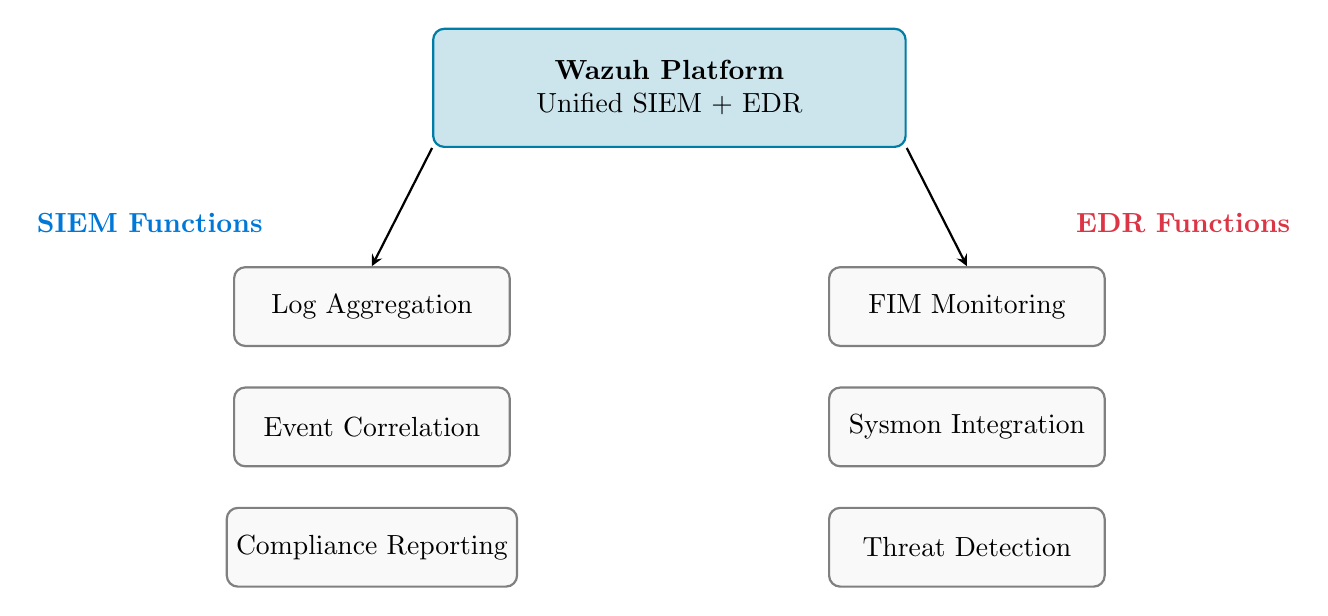
\begin{tikzpicture}[
    box/.style={draw=wazuhblue, thick, rounded corners, minimum width=4cm, minimum height=1.5cm, align=center, fill=blue!5},
    smallbox/.style={draw=gray, thick, rounded corners, minimum width=3.5cm, minimum height=1cm, align=center, fill=gray!5},
    arrow/.style={->, thick, >=stealth}
]

% Wazuh Central
\node[box, minimum width=6cm, fill=wazuhblue!20] (wazuh) {\textbf{Wazuh Platform}\\Unified SIEM + EDR};

% SIEM Features
\node[smallbox, below left=1.5cm and -1cm of wazuh] (siem1) {Log Aggregation};
\node[smallbox, below=0.5cm of siem1] (siem2) {Event Correlation};
\node[smallbox, below=0.5cm of siem2] (siem3) {Compliance Reporting};

% EDR Features
\node[smallbox, below right=1.5cm and -1cm of wazuh] (edr1) {FIM Monitoring};
\node[smallbox, below=0.5cm of edr1] (edr2) {Sysmon Integration};
\node[smallbox, below=0.5cm of edr2] (edr3) {Threat Detection};

% Labels
\node[above left=0.3cm and -0.5cm of siem1, font=\bfseries\color{winblue}] {SIEM Functions};
\node[above right=0.3cm and -0.5cm of edr1, font=\bfseries\color{alertred}] {EDR Functions};

% Arrows
\draw[arrow] (wazuh.south west) -- (siem1.north);
\draw[arrow] (wazuh.south east) -- (edr1.north);

\end{tikzpicture}
\caption{Wazuh Unified SIEM + EDR Architecture}
\label{fig:unified}
\end{figure}

\subsubsection{Demonstrated Integration Benefits}

\begin{itemize}
    \item \textbf{Single Pane of Glass:} Unified dashboard for all security operations
    \item \textbf{Cross-Domain Correlation:} Link endpoint activity with network/system logs
    \item \textbf{Reduced Tool Sprawl:} One platform instead of multiple point solutions
    \item \textbf{Cost-Effective:} Open-source solution with enterprise capabilities
    \item \textbf{FIM Bridge:} File Integrity Monitoring spans both SIEM and EDR domains
    \item \textbf{Enhanced Telemetry:} Sysmon integration provides deep EDR visibility
\end{itemize}

\newpage

% ============================================================
% SECTION 6: IAM/PAM
% ============================================================

\section{Identity and Access Management (IAM) \& Privileged Access Management (PAM)}

\subsection{IAM Concepts Demonstrated}

\subsubsection{Authentication Monitoring}

\begin{table}[H]
\centering
\begin{tabularx}{\textwidth}{|l|l|X|}
\hline
\textbf{Event} & \textbf{ID} & \textbf{Security Value} \\
\hline
Windows Failed Logon & 4625 & Track unauthorized access attempts \\
\hline
SSH Auth Failure & Rule 5710 & Detect brute force attacks \\
\hline
Successful Auth & Various & Establish baseline behavior \\
\hline
\end{tabularx}
\caption{Authentication Monitoring Events}
\end{table}

\subsubsection{Account Lifecycle Management}

\begin{itemize}
    \item \textbf{Windows Event 4720:} User account creation detected and logged
    \item \textbf{Account Modifications:} All changes tracked through audit logs
    \item \textbf{Compliance Value:} Supports joiner/mover/leaver processes
\end{itemize}

\subsubsection{Authorization \& Privilege Changes}

\begin{itemize}
    \item \textbf{Windows Event 4732:} Group membership changes monitored
    \item \textbf{Linux Sudo Tracking:} Full command history with user context
    \item \textbf{Detection:} Unauthorized privilege escalation attempts identified
\end{itemize}

\subsubsection{Identity-Based Threat Detection}

\begin{itemize}
    \item Multiple failed logins indicate credential stuffing attempts
    \item Unusual authentication patterns signal compromised accounts
    \item Lateral movement detection through authentication correlation
\end{itemize}

\subsection{PAM (Privileged Access Management) Relevance}

\subsubsection{Privileged Activity Monitoring}

\begin{table}[H]
\centering
\begin{tabularx}{\textwidth}{|l|X|}
\hline
\textbf{Activity} & \textbf{Monitoring Capability} \\
\hline
Sudo Executions & Logged with timestamp, user, and full command \\
\hline
Windows Admin Actions & Tracked through security event logs \\
\hline
Root/SYSTEM Access & High-severity alerts generated \\
\hline
\end{tabularx}
\caption{Privileged Activity Monitoring}
\end{table}

\subsubsection{Compliance Support}

\begin{itemize}
    \item \textbf{Least Privilege:} Visibility into who uses privileged accounts and when
    \item \textbf{Just-In-Time Access:} Logs validate that privileges used were authorized
    \item \textbf{Audit Trail:} Full documentation for SOX, PCI-DSS, HIPAA compliance
    \item \textbf{Anomaly Detection:} After-hours privileged access flagged
\end{itemize}

\subsection{Lab Demonstration Summary}

\begin{infobox}[IAM/PAM Lab Activities]
\begin{enumerate}
    \item Created user "labuser" on Windows (Event 4720)
    \item Added "labuser" to Administrators group (Event 4732)
    \item Monitored sudo usage for privilege escalation (Rule 5402)
    \item Tracked authentication attempts and failures across platforms
    \item Established complete audit trail for identity-related activities
\end{enumerate}
\end{infobox}

\newpage

% ============================================================
% SECTION 7: THREAT HUNTING
% ============================================================

\section{Threat Hunting - Sample Queries \& Analysis}

\subsection{Query 1: Failed Authentication Analysis}

\begin{infobox}[Objective]
Identify potential brute force attacks or credential stuffing attempts across the infrastructure.
\end{infobox}

\subsubsection{Wazuh Query}

\begin{lstlisting}[style=wazuhquery]
rule.groups:"authentication_failed" AND agent.name:"Linux-Client"
\end{lstlisting}

\subsubsection{Analysis Approach}

\begin{enumerate}
    \item \textbf{Pattern Recognition:} Look for multiple failures from same source IP
    \item \textbf{Timing Analysis:} Check intervals between attempts (automated vs manual)
    \item \textbf{Correlation:} Link with successful authentication after failures
    \item \textbf{User Enumeration:} Investigate which accounts are being targeted
\end{enumerate}

\subsubsection{Detection Indicators}

\begin{itemize}
    \item $>5$ failures within 5 minutes = likely automated attack
    \item Failures for multiple usernames = scanning/enumeration
    \item Geographic anomalies = authentication from unusual locations
\end{itemize}

\subsubsection{Response Actions}

\begin{enumerate}
    \item Block source IP at firewall/security group
    \item Implement account lockout policies
    \item Enable MFA for targeted accounts
    \item Review for any successful authentications from same source
\end{enumerate}

\subsection{Query 2: Privileged Account Activity}

\begin{infobox}[Objective]
Monitor for unauthorized privilege escalation or suspicious administrative activity.
\end{infobox}

\subsubsection{Wazuh Query}

\begin{lstlisting}[style=wazuhquery]
(rule.id:5402 OR data.win.eventdata.eventID:4672) 
AND NOT user.name:"expected_admin"
\end{lstlisting}

\subsubsection{Analysis Approach}

\begin{enumerate}
    \item \textbf{Identify:} All sudo/administrator usage
    \item \textbf{Filter:} Exclude known legitimate administrators
    \item \textbf{Timing:} Check for unusual timing (after-hours, weekends)
    \item \textbf{Correlate:} Link with other suspicious activities
\end{enumerate}

\subsubsection{Detection Indicators}

\begin{itemize}
    \item Privilege escalation by non-admin users
    \item Service accounts used interactively
    \item Unusual commands with elevated privileges
    \item Privilege use from unexpected systems/IPs
\end{itemize}

\subsubsection{Response Actions}

\begin{enumerate}
    \item Validate whether privilege use was authorized
    \item Review command history for malicious activity
    \item Disable compromised accounts immediately
    \item Initiate incident response if unauthorized
\end{enumerate}

\subsection{Query 3: Process Anomaly Detection (EDR)}

\begin{infobox}[Objective]
Identify suspicious process execution patterns indicating malware or living-off-the-land attacks.
\end{infobox}

\subsubsection{Wazuh Query}

\begin{lstlisting}[style=wazuhquery]
data.win.system.eventID:1 AND 
(data.win.eventdata.commandLine:(*powershell* AND *-enc*) OR 
 data.win.eventdata.commandLine:(*cmd* AND */c* AND *certutil*))
\end{lstlisting}

\subsubsection{Analysis Approach}

\begin{enumerate}
    \item \textbf{Encoded Commands:} Look for encoded PowerShell (common in malware)
    \item \textbf{Process Relationships:} Identify unusual parent-child patterns
    \item \textbf{LOLBins:} Check for system binaries used maliciously
    \item \textbf{Network Correlation:} Link process creation with network connections (Sysmon Event 3)
\end{enumerate}

\subsubsection{Detection Indicators}

\begin{itemize}
    \item PowerShell with encoded commands (-enc, -EncodedCommand)
    \item cmd.exe spawning unusual children (certutil, bitsadmin, wmic)
    \item Processes running from temporary directories
    \item Suspicious parent processes (e.g., Excel spawning PowerShell)
    \item Processes with network connections to unknown IPs
\end{itemize}

\subsubsection{Response Actions}

\begin{enumerate}
    \item Isolate affected endpoint immediately
    \item Collect process memory dump for analysis
    \item Check file hashes against threat intelligence
    \item Review network logs for C2 communication
    \item Initiate full forensic investigation
\end{enumerate}

\subsection{Threat Hunting Best Practices}

\begin{table}[H]
\centering
\begin{tabularx}{\textwidth}{|l|X|}
\hline
\textbf{Practice} & \textbf{Description} \\
\hline
Time Correlation & Look for events within short timeframes \\
\hline
Baseline Normal & Understand typical activity before hunting anomalies \\
\hline
Pivot on Indicators & One suspicious event often leads to others \\
\hline
Document Findings & Maintain a hunting journal with queries and results \\
\hline
Continuous Improvement & Refine queries based on findings and new threats \\
\hline
\end{tabularx}
\caption{Threat Hunting Best Practices}
\end{table}

\newpage

% ============================================================
% CONCLUSION
% ============================================================

\section{Conclusion}

This lab successfully demonstrated the implementation of a cloud-based Wazuh SIEM/EDR platform on AWS infrastructure. Key accomplishments include:

\subsection{Technical Achievements}

\begin{itemize}
    \item Deployed a complete monitoring infrastructure with proper network segmentation
    \item Successfully enrolled and monitored both Linux and Windows agents
    \item Captured and analyzed real security events including:
    \begin{itemize}
        \item SSH brute force attacks
        \item Privilege escalation activities
        \item File integrity changes
        \item Windows authentication events
        \item Process-level EDR telemetry via Sysmon
    \end{itemize}
\end{itemize}

\subsection{Security Concepts Validated}

\begin{itemize}
    \item \textbf{SIEM Capabilities:} Centralized log aggregation, correlation, and alerting
    \item \textbf{EDR Capabilities:} Deep endpoint visibility with process and file monitoring
    \item \textbf{IAM/PAM:} Identity and privilege monitoring for compliance and security
    \item \textbf{Threat Hunting:} Practical queries for proactive threat detection
\end{itemize}

\subsection{Operational Value}

Wazuh provides a cost-effective, open-source solution that combines SIEM and EDR capabilities in a unified platform. This lab demonstrates its applicability for:

\begin{itemize}
    \item Small to medium enterprise security monitoring
    \item Cloud-native security operations
    \item Compliance and audit requirements
    \item Security Operations Center (SOC) implementations
\end{itemize}

\begin{infobox}[Key Takeaway]
The integration of SIEM and EDR capabilities in a single platform like Wazuh provides comprehensive security visibility while reducing operational complexity and cost—essential for modern security operations in cloud environments.
\end{infobox}

\end{document}
